%10_adverserial_search.tex
%notes for the course PandA2 COMS10001 taught at the University of Bristol
%2016-7 Conor Houghton conor.houghton@bristol.ac.uk

%To the extent possible under law, the author has dedicated all copyright 
%and related and neighboring rights to these notes to the public domain 
%worldwide. These notes are distributed without any warranty. 

\documentclass[11pt,a4paper]{scrartcl}
\typearea{12}
\usepackage{graphicx}
\usepackage{listings}
\usepackage{tikz-qtree}
\lstset{language=C}
\pagestyle{headings}
\markright{COMS10001 - PandA2 10\_adverserial\_search - Conor}
\begin{document}

\subsection*{10 - adverserial search}

\begin{figure}
\begin{center}
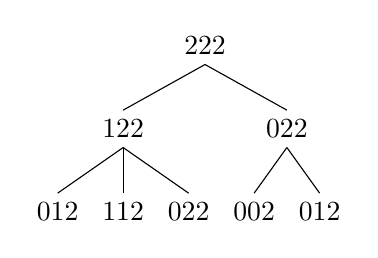
\begin{tikzpicture}
\Tree
[.222   
  [.122
    [.012 ]
    [.112 ]
    [.022 ]
  ]
  [.022
    [.002 ]
    [.012 ]
  ]
]
\end{tikzpicture}
\end{center}
\caption{}
\end{figure}


\end{document}
